\documentclass[11pt]{article}

\usepackage[margin=1in]{geometry}
\usepackage{graphicx}
\usepackage{booktabs}
\usepackage{longtable}
\usepackage{array}
\usepackage{multirow}
\usepackage{caption}
\usepackage{subcaption}
\usepackage{microtype}
\usepackage{xcolor}
\usepackage{hyperref}
\usepackage{xurl}
\usepackage{listings}

\hypersetup{
  colorlinks=true,
  linkcolor=blue,
  citecolor=blue,
  urlcolor=blue
}

\lstset{
  basicstyle=\ttfamily\small,
  columns=fullflexible,
  breaklines=true,
  frame=single,
  rulecolor=\color{black!15},
  xleftmargin=0.5em,
  xrightmargin=0.5em
}

% ---- tighter longtable helper ----
\newenvironment{tightlongtable}[1]{%
  \begin{center}
  \footnotesize
  \setlength{\tabcolsep}{3.2pt}% column padding
  \renewcommand{\arraystretch}{0.92}% row height
  \setlength{\LTleft}{0pt}% remove left indent
  \setlength{\LTright}{0pt}% remove right indent
  \begin{longtable}{#1}
}{%
  \end{longtable}
  \end{center}
}

\title{Qwen3.5: Towards Native Multimodal Agents\\\large Reformatted from the official release materials}
\author{Qwen Team (original release) \and This \LaTeX{} version: autogenerated from public materials}
\date{February 2026}

\begin{document}
\maketitle

\begin{abstract}
Qwen3.5 is a native multimodal mixture-of-experts (MoE) foundation model designed for agentic workloads that require reasoning over language, images, and interactive tool use.
According to the official release materials, Qwen3.5 combines (i) early-fusion multimodal pretraining, (ii) an efficient hybrid architecture based on Gated Delta Networks with sparse MoE routing, and (iii) reinforcement learning (RL) scaled to large numbers of agent environments.
This document reorganizes the public release content into a self-contained \LaTeX{} paper, while preserving the original tables and figures.\cite{qwen35blog,qwen35hf}
\end{abstract}

\begin{figure}[htbp]
  \centering
  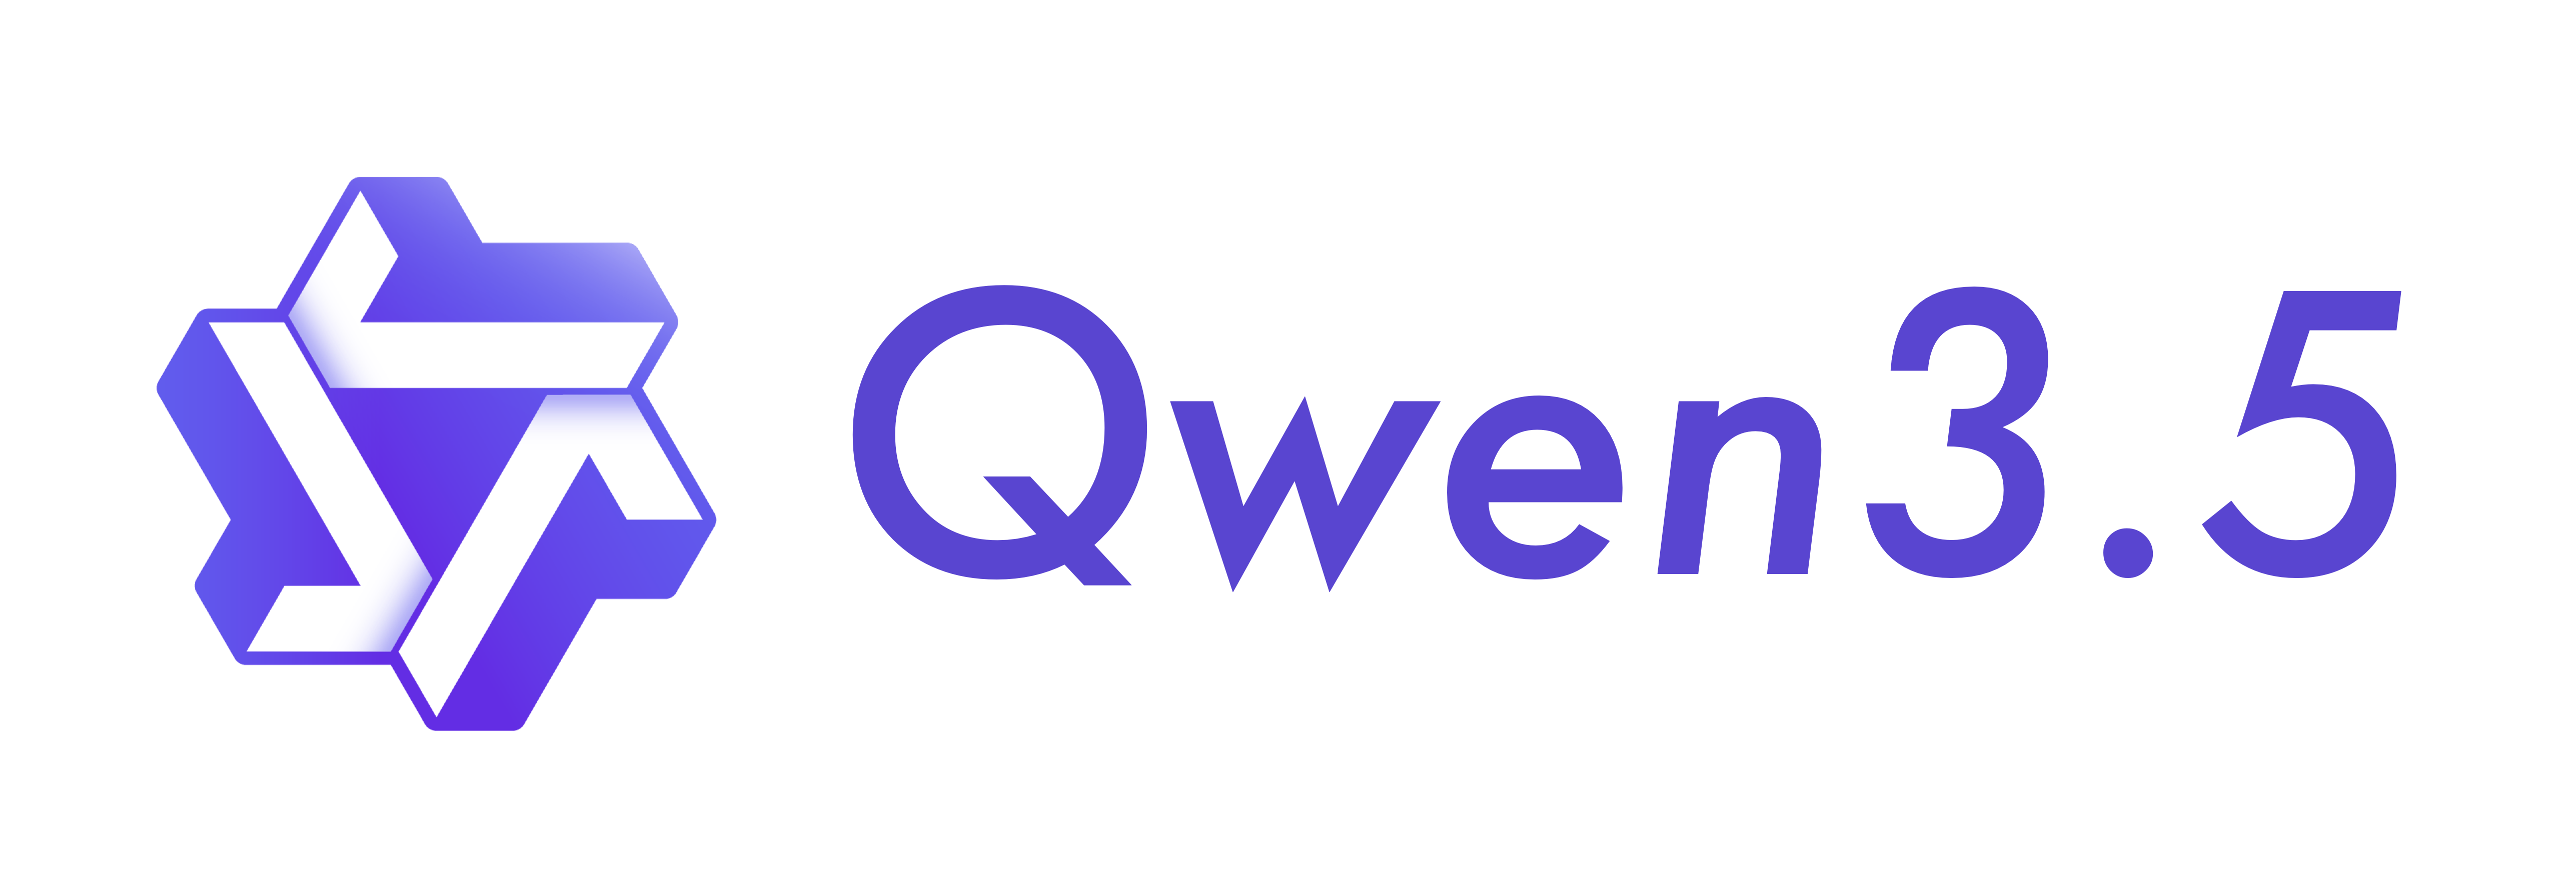
\includegraphics[width=0.44\linewidth]{figures/logo_qwen3_5.png}
  \caption{Qwen3.5 logo used in the official release materials.\cite{qwen35hf}}
  \label{fig:logo}
\end{figure}

\begin{figure}[htbp]
  \centering
  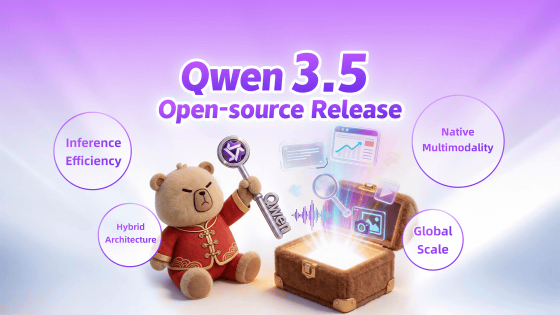
\includegraphics[width=\linewidth]{figures/release_banner.png}
  \caption{Release banner screenshot from public release reporting.\cite{gigazine_qwen35}}
  \label{fig:release_banner}
\end{figure}

\section{Introduction}
Recent ``agentic'' applications increasingly require models to (a) interpret multimodal inputs, (b) plan multi-step actions, and (c) interact with external tools under long contexts.
The Qwen3.5 release positions the model family as an attempt to unify these requirements in a native multimodal foundation model.\cite{qwen35blog}
This paper-like write-up focuses on the first open-weight release, \texttt{Qwen3.5-397B-A17B}, and summarizes its architecture, capabilities, and benchmark results as reported by the authors.\cite{qwen35hf}

\section{Model overview}
The released checkpoint is described as a causal language model with a vision encoder and a sparse MoE backbone.\cite{qwen35hf}
Key properties are summarized in \autoref{tab:config}.

\begin{table}[htbp]
\small
\centering
\caption{Selected configuration details for \texttt{Qwen3.5-397B-A17B} as reported in the official model card.\cite{qwen35hf}}
\label{tab:config}
\scalebox{0.90}{
\setlength{\tabcolsep}{0.8mm}
\begin{tabular}{@{}ll@{}}
\toprule
Item & Value \\
\midrule
Total parameters & 397B \\
Active parameters & 17B \\
Layers & 60 \\
Hidden dimension & 4096 \\
Vocabulary size & 248{,}320 (padded) \\
MoE experts & 512 (10 routed + 1 shared activated) \\
Context length & 262{,}144 native; extensible to 1{,}010{,}000 \\
Backbone & 15 $\times$ [3 $\times$ (Gated DeltaNet $\rightarrow$ MoE) + 1 $\times$ (Gated Attention $\rightarrow$ MoE)] \\
\bottomrule
\end{tabular}
}
\end{table}

\section{Design highlights (from the release materials)}
The official release emphasizes the following themes: \cite{qwen35blog,qwen35hf}
\begin{itemize}
  \item \textbf{Unified vision--language foundation.} Early-fusion training on large multimodal corpora aims to align visual understanding with language reasoning.
  \item \textbf{Efficient hybrid architecture.} Gated Delta Networks and sparse MoE routing are used to improve throughput and reduce inference overhead.
  \item \textbf{Scalable RL generalization.} RL is reported to be scaled across large collections of tool-using agent environments with progressively more complex task distributions.
  \item \textbf{Broad multilingual coverage.} The release materials claim support for 201 languages and dialects.
\end{itemize}

\begin{figure}[htbp]
  \centering
  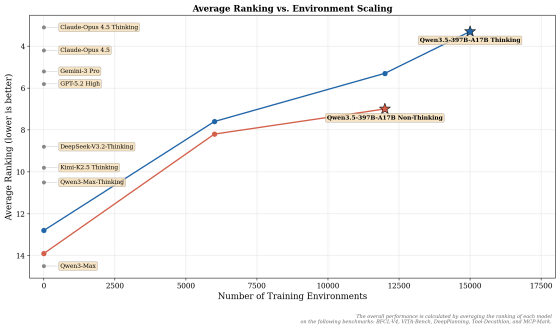
\includegraphics[width=0.92\linewidth]{figures/env_scaling.png}
  \caption{Example figure on RL environment scaling reproduced in public release reporting.\cite{gigazine_qwen35}}
  \label{fig:env_scaling}
\end{figure}

\section{Benchmarks}
\subsection{Summary figures}
\autoref{fig:score} reproduces the benchmark summary figure from the official release repository.\cite{qwen35hf}

\begin{figure}[htbp]
  \centering
  \includegraphics[width=\linewidth]{figures/qwen3_5_score.png}
  \caption{Benchmark score overview for \texttt{Qwen3.5-397B-A17B} as provided in the official release materials.\cite{qwen35hf}}
  \label{fig:score}
\end{figure}

\begin{figure}[htbp]
  \centering
  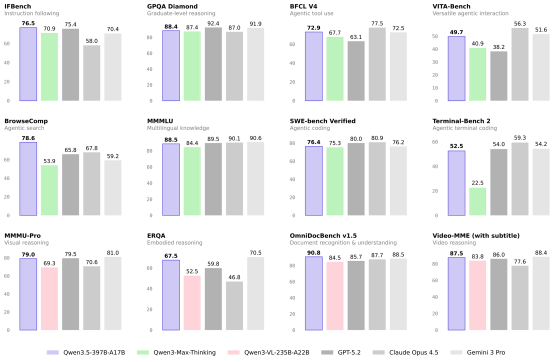
\includegraphics[width=0.95\linewidth]{figures/bench_mini_panels.png}
  \caption{Additional benchmark panel screenshot reproduced in public release reporting.\cite{gigazine_qwen35}}
  \label{fig:bench_panels}
\end{figure}

\begin{figure}[htbp]
  \centering
  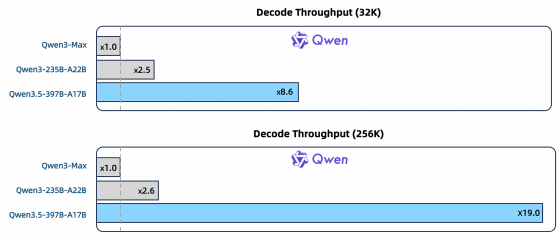
\includegraphics[width=0.92\linewidth]{figures/decode_throughput.png}
  \caption{Decode throughput chart reproduced in public release reporting.\cite{gigazine_qwen35}}
  \label{fig:throughput}
\end{figure}

\subsection{Language benchmarks}
\autoref{tab:bench-language} lists the detailed language results extracted from the official model card (HTML table preserved and converted into \LaTeX{}).\cite{qwen35hf}

\begin{tightlongtable}{p{0.20\linewidth} r r r r r r}
  \caption{Language benchmark results reported in the Qwen3.5 model card.}\label{tab:bench-language}\\
\toprule
Metric & GPT5.2 & Claude 4.5 Opus & Gemini-3 Pro & Qwen3-Max-Thinking & K2.5-1T-A32B & Qwen3.5-397B-A17B \\
\midrule
\endfirsthead
\toprule
Metric & GPT5.2 & Claude 4.5 Opus & Gemini-3 Pro & Qwen3-Max-Thinking & K2.5-1T-A32B & Qwen3.5-397B-A17B \\
\midrule
\endhead
\bottomrule
\endfoot

\multicolumn{7}{l}{\textbf{Knowledge}}\\
MMLU-Pro & 87.4 & 89.5 & 89.8 & 85.7 & 87.1 & 87.8 \\
MMLU-Redux & 95.0 & 95.6 & 95.9 & 92.8 & 94.5 & 94.9 \\
SuperGPQA & 67.9 & 70.6 & 74.0 & 67.3 & 69.2 & 70.4 \\
C-Eval & 90.5 & 92.2 & 93.4 & 93.7 & 94.0 & 93.0 \\
\addlinespace[0.4ex]
\multicolumn{7}{l}{\textbf{Instruction Following}}\\
IFEval & 94.8 & 90.9 & 93.5 & 93.4 & 93.9 & 92.6 \\
IFBench & 75.4 & 58.0 & 70.4 & 70.9 & 70.2 & 76.5 \\
MultiChallenge & 57.9 & 54.2 & 64.2 & 63.3 & 62.7 & 67.6 \\
\addlinespace[0.4ex]
\multicolumn{7}{l}{\textbf{Long Context}}\\
AA-LCR & 72.7 & 74.0 & 70.7 & 68.7 & 70.0 & 68.7 \\
LongBench v2 & 54.5 & 64.4 & 68.2 & 60.6 & 61.0 & 63.2 \\
\addlinespace[0.4ex]
\multicolumn{7}{l}{\textbf{STEM}}\\
GPQA & 92.4 & 87.0 & 91.9 & 87.4 & 87.6 & 88.4 \\
HLE & 35.5 & 30.8 & 37.5 & 30.2 & 30.1 & 28.7 \\
HLE-Verified\textsuperscript{1} & 43.3 & 38.8 & 48 & 37.6 & -- & 37.6 \\
\addlinespace[0.4ex]
\multicolumn{7}{l}{\textbf{Reasoning}}\\
LiveCodeBench v6 & 87.7 & 84.8 & 90.7 & 85.9 & 85.0 & 83.6 \\
HMMT Feb 25 & 99.4 & 92.9 & 97.3 & 98.0 & 95.4 & 94.8 \\
HMMT Nov 25 & 100 & 93.3 & 93.3 & 94.7 & 91.1 & 92.7 \\
IMOAnswerBench & 86.3 & 84.0 & 83.3 & 83.9 & 81.8 & 80.9 \\
AIME26 & 96.7 & 93.3 & 90.6 & 93.3 & 93.3 & 91.3 \\
\addlinespace[0.4ex]
\multicolumn{7}{l}{\textbf{General Agent}}\\
BFCL-V4 & 63.1 & 77.5 & 72.5 & 67.7 & 68.3 & 72.9 \\
TAU2-Bench & 87.1 & 91.6 & 85.4 & 84.6 & 77.0 & 86.7 \\
VITA-Bench & 38.2 & 56.3 & 51.6 & 40.9 & 41.9 & 49.7 \\
DeepPlanning & 44.6 & 33.9 & 23.3 & 28.7 & 14.5 & 34.3 \\
Tool Decathlon & 43.8 & 43.5 & 36.4 & 18.8 & 27.8 & 38.3 \\
MCP-Mark & 57.5 & 42.3 & 53.9 & 33.5 & 29.5 & 46.1 \\
\addlinespace[0.4ex]
\multicolumn{7}{l}{\textbf{Search Agent\textsuperscript{3}}}\\
HLE w/ tool & 45.5 & 43.4 & 45.8 & 49.8 & 50.2 & 48.3 \\
BrowseComp & 65.8 & 67.8 & 59.2 & 53.9 & --/74.9 & 69.0/78.6 \\
BrowseComp-zh & 76.1 & 62.4 & 66.8 & 60.9 & -- & 70.3 \\
WideSearch & 76.8 & 76.4 & 68.0 & 57.9 & 72.7 & 74.0 \\
Seal-0 & 45.0 & 47.7 & 45.5 & 46.9 & 57.4 & 46.9 \\
\addlinespace[0.4ex]
\multicolumn{7}{l}{\textbf{Multilingualism}}\\
MMMLU & 89.5 & 90.1 & 90.6 & 84.4 & 86.0 & 88.5 \\
MMLU-ProX & 83.7 & 85.7 & 87.7 & 78.5 & 82.3 & 84.7 \\
NOVA-63 & 54.6 & 56.7 & 56.7 & 54.2 & 56.0 & 59.1 \\
INCLUDE & 87.5 & 86.2 & 90.5 & 82.3 & 83.3 & 85.6 \\
Global PIQA & 90.9 & 91.6 & 93.2 & 86.0 & 89.3 & 89.8 \\
PolyMATH & 62.5 & 79.0 & 81.6 & 64.7 & 43.1 & 73.3 \\
WMT24++ & 78.8 & 79.7 & 80.7 & 77.6 & 77.6 & 78.9 \\
MAXIFE & 88.4 & 79.2 & 87.5 & 84.0 & 72.8 & 88.2 \\
\addlinespace[0.4ex]
\multicolumn{7}{l}{\textbf{Coding Agent}}\\
SWE-bench Verified & 80.0 & 80.9 & 76.2 & 75.3 & 76.8 & 76.4 \\
SWE-bench Multilingual & 72.0 & 77.5 & 65.0 & 66.7 & 73.0 & 69.3 \\
SecCodeBench & 68.7 & 68.6 & 62.4 & 57.5 & 61.3 & 68.3 \\
Terminal Bench 2 & 54.0 & 59.3 & 54.2 & 22.5 & 50.8 & 52.5 \\
\addlinespace[0.4ex]
\end{tightlongtable}

\subsection{Vision--language benchmarks}
\autoref{tab:bench-vl} lists the detailed vision--language results extracted from the official model card (HTML table preserved and converted into \LaTeX{}).\cite{qwen35hf}

\begin{tightlongtable}{p{0.10\linewidth} r r r r r r}
\caption{Vision-language benchmark results reported in the Qwen3.5 model card.}\label{tab:bench-vl}\\
\toprule
Metric & GPT5.2 & Claude 4.5 Opus & Gemini-3 Pro & Qwen3-VL-235B-A22B & K2.5-1T-A32B & Qwen3.5-397B-A17B \\
\midrule
\endfirsthead
\toprule
Metric & GPT5.2 & Claude 4.5 Opus & Gemini-3 Pro & Qwen3-VL-235B-A22B & K2.5-1T-A32B & Qwen3.5-397B-A17B \\
\midrule
\endhead
\bottomrule
\endfoot
\multicolumn{7}{l}{\textbf{STEM and Puzzle}}\\
MMMU & 86.7 & 80.7 & 87.2 & 80.6 & 84.3 & 85.0 \\
MMMU-Pro & 79.5 & 70.6 & 81.0 & 69.3 & 78.5 & 79.0 \\
MathVision & 83.0 & 74.3 & 86.6 & 74.6 & 84.2 & 88.6 \\
Mathvista(mini) & 83.1 & 80.0 & 87.9 & 85.8 & 90.1 & 90.3 \\
We-Math & 79.0 & 70.0 & 86.9 & 74.8 & 84.7 & 87.9 \\
DynaMath & 86.8 & 79.7 & 85.1 & 82.8 & 84.4 & 86.3 \\
ZEROBench & 9 & 3 & 10 & 4 & 9 & 12 \\
ZEROBench\_sub & 33.2 & 28.4 & 39.0 & 28.4 & 33.5 & 41.0 \\
BabyVision & 34.4 & 14.2 & 49.7 & 22.2 & 36.5 & 52.3/43.3 \\
\addlinespace[0.4ex]
\multicolumn{7}{l}{\textbf{General VQA}}\\
RealWorldQA & 83.3 & 77.0 & 83.3 & 81.3 & 81.0 & 83.9 \\
MMStar & 77.1 & 73.2 & 83.1 & 78.7 & 80.5 & 83.8 \\
HallusionBench & 65.2 & 64.1 & 68.6 & 66.7 & 69.8 & 71.4 \\
MMBenchEN-DEV-v1.1 & 88.2 & 89.2 & 93.7 & 89.7 & 94.2 & 93.7 \\
SimpleVQA & 55.8 & 65.7 & 73.2 & 61.3 & 71.2 & 67.1 \\
\addlinespace[0.4ex]
\multicolumn{7}{l}{\textbf{Text Recognition and Document Understanding}}\\
OmniDocBench1.5 & 85.7 & 87.7 & 88.5 & 84.5 & 88.8 & 90.8 \\
CharXiv(RQ) & 82.1 & 68.5 & 81.4 & 66.1 & 77.5 & 80.8 \\
MMLongBench-Doc & -- & 61.9 & 60.5 & 56.2 & 58.5 & 61.5 \\
CC-OCR & 70.3 & 76.9 & 79.0 & 81.5 & 79.7 & 82.0 \\
AI2D\_TEST & 92.2 & 87.7 & 94.1 & 89.2 & 90.8 & 93.9 \\
OCRBench & 80.7 & 85.8 & 90.4 & 87.5 & 92.3 & 93.1 \\
\addlinespace[0.4ex]
\multicolumn{7}{l}{\textbf{Spatial Intelligence}}\\
ERQA & 59.8 & 46.8 & 70.5 & 52.5 & -- & 67.5 \\
CountBench & 91.9 & 90.6 & 97.3 & 93.7 & 94.1 & 97.2 \\
RefCOCO(avg) & -- & -- & 84.1 & 91.1 & 87.8 & 92.3 \\
ODInW13 & -- & -- & 46.3 & 43.2 & -- & 47.0 \\
EmbSpatialBench & 81.3 & 75.7 & 61.2 & 84.3 & 77.4 & 84.5 \\
RefSpatialBench & -- & -- & 65.5 & 69.9 & -- & 73.6 \\
LingoQA & 68.8 & 78.8 & 72.8 & 66.8 & 68.2 & 81.6 \\
V* & 75.9 & 67.0 & 88.0 & 85.9 & 77.0 & 95.8/91.1 \\
Hypersim & -- & -- & -- & 11.0 & -- & 12.5 \\
SUNRGBD & -- & -- & -- & 34.9 & -- & 38.3 \\
Nuscene & -- & -- & -- & 13.9 & -- & 16.0 \\
\addlinespace[0.4ex]
\multicolumn{7}{l}{\textbf{Video Understanding}}\\
VideoMME(w sub.) & 86 & 77.6 & 88.4 & 83.8 & 87.4 & 87.5 \\
VideoMME(w/o sub.) & 85.8 & 81.4 & 87.7 & 79.0 & 83.2 & 83.7 \\
VideoMMMU & 85.9 & 84.4 & 87.6 & 80.0 & 86.6 & 84.7 \\
MLVU (M-Avg) & 85.6 & 81.7 & 83.0 & 83.8 & 85.0 & 86.7 \\
MVBench & 78.1 & 67.2 & 74.1 & 75.2 & 73.5 & 77.6 \\
LVBench & 73.7 & 57.3 & 76.2 & 63.6 & 75.9 & 75.5 \\
MMVU & 80.8 & 77.3 & 77.5 & 71.1 & 80.4 & 75.4 \\
\addlinespace[0.4ex]
\multicolumn{7}{l}{\textbf{Visual Agent}}\\
ScreenSpot Pro & -- & 45.7 & 72.7 & 62.0 & -- & 65.6 \\
OSWorld-Verified & 38.2 & 66.3 & -- & 38.1 & 63.3 & 62.2 \\
AndroidWorld & -- & -- & -- & 63.7 & -- & 66.8 \\
\addlinespace[0.4ex]
\multicolumn{7}{l}{\textbf{Medical VQA}}\\
SLAKE & 76.9 & 76.4 & 81.3 & 54.7 & 81.6 & 79.9 \\
PMC-VQA & 58.9 & 59.9 & 62.3 & 41.2 & 63.3 & 64.2 \\
MedXpertQA-MM & 73.3 & 63.6 & 76.0 & 47.6 & 65.3 & 70.0 \\
\addlinespace[0.4ex]
\end{tightlongtable}

\section{Usage and deployment notes}
The release materials provide example commands for serving the model locally via multiple frameworks.\cite{qwen35hf}
Below we reproduce representative snippets.

\subsection{Hugging Face Transformers (serving)}
\begin{lstlisting}[language=bash]
transformers serve --port 8000 --continuous-batching
# OpenAI-compatible endpoint:
#   http://localhost:8000/v1
\end{lstlisting}

\subsection{SGLang}
\begin{lstlisting}[language=bash]
python -m sglang.launch_server \
  --model-path Qwen/Qwen3.5-397B-A17B \
  --port 8000 --tp-size 8 \
  --context-length 262144 \
  --reasoning-parser qwen3
\end{lstlisting}

\subsection{vLLM}
\begin{lstlisting}[language=bash]
vllm serve Qwen/Qwen3.5-397B-A17B \
  --port 8000 \
  --tensor-parallel-size 8 \
  --max-model-len 262144 \
  --reasoning-parser qwen3
\end{lstlisting}

% \newpage
\begin{thebibliography}{9}
\bibitem{qwen35blog}
Qwen Team.
\newblock {Qwen3.5}: Towards Native Multimodal Agents.
\newblock February 2026.
\newblock \url{https://qwen.ai/blog?id=qwen3.5}.

\bibitem{qwen35hf}
Qwen Team.
\newblock {Qwen3.5-397B-A17B} Model Card.
\newblock 2026.
\newblock \url{https://huggingface.co/Qwen/Qwen3.5-397B-A17B}.

\bibitem{gigazine_qwen35}
GIGAZINE.
\newblock Open source release of {Qwen3.5-397B-A17B} and benchmark summaries (includes screenshots of the release materials).
\newblock February 2026.
\newblock \url{https://gigazine.net/news/20260217-qwen3-5-397b-a17b/}.

\end{thebibliography}

\end{document}
